\documentclass[UTF8]{ctexart}
\usepackage{graphicx}
\usepackage{amsmath}
\begin{document}

\title{隐马尔可夫模型}
\author{庞海天}
\maketitle
\section{隐马尔科夫模型介绍}
我们到现在为止所考虑的所有马尔科夫模型都具有可见的状态,也就是说所有的状态序列是知道的。因此我们可以将这些模型称为显马尔科夫模型。在这一章我们考虑状态序列是不知道的,但是可以由一系列动态过程的观测来进行推测。我们将这种模型称为隐马尔科夫模型。

隐马尔科夫模型假设正在进行的过程是一个马尔科夫链,它的内部状态隐含在观察之中。通常会假设系统中状态的数量和状态转移概率是知道的。因此隐马尔科夫模型的每个状态就有两个与之相关的参数:

$\bullet$用来描述统一状态的不同输出概率的符号发射概率。

$\bullet$用来描述从当前状态转移到一个新的状态的概率的转移概率矩阵

显马尔科夫模型通常在很多应用环境的建模中受限。它们的限制来自它们假设事先知道系统内部的动态并且可以通过某些协议系统的演化。然而对于一些不满足这两个假设的应用场景,隐马尔科夫就可以使用了。

\section{隐马尔科夫初步}
隐马尔科夫模型是一个符合的随机过程,其中有一个不可见的随机过程,而有另外一个可观察的随机过程。因此如果$S={S_n,n=1,2,...}$是一个马尔科夫过程并且$\Omega={\Omega_k,k=1,2,...}$是S的函数,就可以说S是一个通过$\Omega$观察的隐马尔科夫模型,我们可以
写做$\Omega_k=f(S_k)$。这样我们可以认为S是隐状态过程而$\Omega$是可以被观察的信号过程。

隐马尔科夫模型通常由一个五元组定义$(S,\Omega,P,\Phi,\pi)$其中

$\bullet S={s_1,s_2,...,s_N}$是一组有限的N个状态

$\bullet \Omega={o_1,o_2,...,o_M}$是一组有限的M个信号

$\bullet P={p_{ij}}$是一组状态转移概率矩阵,其中$p_{ij}$是系统由状态$s_i$转移到状态$s_j$的概率

$\bullet \Phi={\phi_i(o_k)}$是信号观察概率,其中${\phi_i(o_k)}$是系统处于状态$s_i$时,发射出信号$o_k$的概率

$\bullet \pi={\pi_i}$是初始状态概率,也就是说$\pi_i$是系统在状态$s_i$开始的概率

通常习惯用$\lambda = (P,\Phi,\pi)$来代表隐马尔科夫模型的参数。

\section{隐马尔科夫的假设}

令$Q=(q_t)$来代表在区间$0\le t\le T$中的因状态序列,其中$q_t\in S$。在隐马尔科夫模型分析当中,一共有三个重要的假设:

1.马氏性:该假设说明下一个状态仅依赖当前状态,而与之前的状态无关。
\begin{center}
$\begin{aligned}
P(q_{t+1}=j|q_t=i,q_{t-1}=l,...,q_0=n) \\
=P(q_{t+1}=j|q_t=i)=p_{ij}
\end{aligned}
$
\end{center}
2.增量平稳性:这一假设说明状态转移概率矩阵与转移发生的实际时间是独立的。也就是说,对任意两个时间$t_1$和$t_2$,

$P(q_{t_1+1}=j|q_{t_1}=i)=P(q_{t_2+1}=j|q_{t_2}=i)=p_{ij}$

3.观察独立性:这假设当前观测或者输出与之前的观察是独立的。所以如果我们有观察序列$O=v_1,v_2,...,v_T$,那么

$P(O|q_1,q_2,...,q_T,\lambda) = \prod_{t=1}^T P(v_t|q_t,\lambda)$

有这些假设,我们可以得到联合概率分布$P(Q,O)$:

\begin{center}
$P(Q,O)=\prod_{t=1}^T P(q_t|q_{t-1})P(v_t|q_t)$
\end{center}

其中$P(q_1|q_0)\equiv P(q_1)$。


\section{三个基本问题}

在隐马尔科夫模型中有三个基本问题:

1、评价问题:已知一个模型$\lambda=(P,\Phi,\pi)$和一个长度为T的观察序列$O=v_1,v_2,...,v_T$,其中$v_i\in \Omega$,我们如何高效的计算出模型生成观测序列的概率呢?即$P[O|\lambda]$等于多少?

2、解码问题:已知一个模型$\lambda=(P,\Phi,\pi)$,最有可能生成一个已知的观测状态序列的隐状态序列是什么?我们需要找到$Q^*=arg max_QP[Q,O|\lambda]$,其中Q是隐状态序列。

3、学习问题:已知一系列观测序列,找到能够最好地解释该序列的隐马尔科夫模型。也就是说,找到$\lambda^*=arg max_\lambda P[O|\lambda]$。换一种说法,这个问题就是已知观测序列,估计最有可能的隐马尔科夫模型的参数。

\section{解决方法}

对于不同的基本问题,我们有不同的解决方法。评价问题通常用前向算法和后向算法来解。解码问题通常用Viterbi算法来解。学习问题通常用Baum-Welch算法来解。下面本节将介绍这些算法。

\subsection{评价问题与forward and backward algorithm}

考虑一个模型$\lambda=(P,\Phi,\pi)$和一个已知的观测序列$O=o_1,o_2...,o_T$。我们要计算$P[O|\lambda]$,已知一个模型的情况下产生观测序列的概率。

\begin{center}
$P[O|\lambda]=\sum_QP[O|Q,\lambda]P[Q|\lambda]$
\end{center}

其中$Q=q_1,q_2,...,q_T$是一个确定的序列,$P[O|Q,\lambda]$是观测序列O关于特定状态序列Q的条件概率,$P[Q|\lambda]$是一个特定模型的状态序列出现的概率。因为我们假设观测是独立的,这两个概率可以如下表示:

\begin{center}
$
\begin{aligned}
P[O|Q,\lambda]=\prod _{t=1}^TP[o_t|q_t,\lambda]=\phi_{q_1}(o_1)\phi_{q_2}(o_2)...\phi_{q_T}(o_T) \\
P[Q|\lambda]=\pi_{q_1}p_{q_1q_2}p_{q_2q_3}...p_{q_{T-1}q_T}\end{aligned}$
\end{center}

于是,我们可以得到:

\begin{center}
$
\begin{aligned}
P[O|\lambda]=\sum_QP[O|Q,\lambda]P[Q|\lambda]\\
=\sum_{q_1,...,q_T}\pi_{q_1}\phi_{q_1}(o_1)p_{q_1q_2}\phi_{q_2}(o_2)p_{q_2q_3}...p_{q_{T-1}q_T}\phi_{q_T}(o_T)\end{aligned}$
\end{center}

在前面的观察中,首先,我们可以得知长度为T的可能路径的数量为$N^T$,这意味着需要解的等式数量是T的指数倍数。而且用这种直接的获取$P[O|\lambda]$的方法需要$2TN^T$次计算。所以,即使N和T的数量很小,计算量还是很大的。例如,我们假设$N=3,T=100$,需要进行的计算数量为$2\times 100\times 3^100 \approx 10^50$。由于这个原因我们需要一个更加有效率的算法来解评价问题。下面我们将介绍前向算法。


\begin{figure}[htbp]
\centering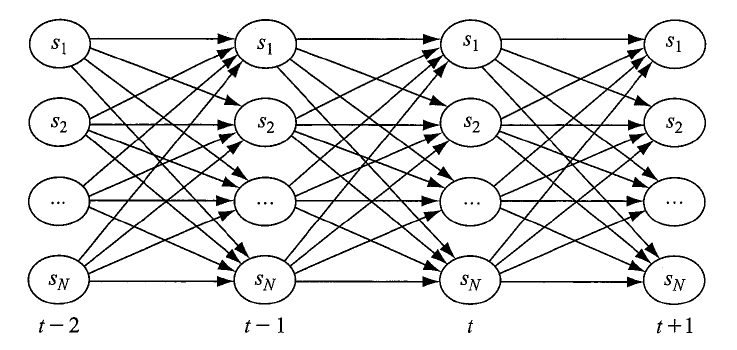
\includegraphics[width=3.5in]{f114}
\caption{前向算法的交织}\label{fig:1}
\end{figure}


一个重要的观察结果是直接方法计算$P[O|\lambda]$的计算量有很多的冗余计算。为了减少计算复杂度,我们缓存计算的结果。在每个时间步长中,缓存作为状态之间的交织状态被执行,如图1。状态的交织记录所有的结束在某个时间某个状态的初始隐马尔科夫过程的子路径的概率。这使得更长的子路径的概率可以由短的子路径的概率计算得到。

前向概率变量$\alpha_t(i)$如下定义:

\begin{center}
$
\alpha_t(i)=P[o_1,o_2,...,o_t,q_t=s_i|\lambda]\quad t=1,...,T;i=1,...,N
$
\end{center}

这就是说,$\alpha_t(i)$是观察到序列$\{o_1,o_2,...,o_t\}$之后,在t时刻位于状态$s_i$的概率。它通过对一个交织节点将所有的输入弧的概率进行加和得到。因为:

\begin{center}
$
\begin{aligned}
P[O|\lambda]=P[o_1,o_2,...,o_t,q_t=s_i|\lambda]\\
=P[o_t|o_1,o_2,...,o_{t-1},q_t=s_i,\lambda]P[o_1,o_2,...,o_{t-1},q_t=s_i|\lambda]\\
=P[o_t|q_t=s_i,\lambda]P[o_1,o_2,...,o_{t-1},q_t=s_i|\lambda]\\
=P[o_t|q_t=s_i,\lambda]\sum_{s_j\in S}P[q_t=s_i|q_{t-1}=s_j,\lambda]P[o_1,o_2,...,o_{t-1},q_{t-1}=s_j|\lambda]\\
=\phi_i(o_t)\sum_{j=1}^Np_{ji}\alpha_{t-1}(j)\quad 1\le t\le T
\end{aligned}$
\end{center}

其中我们假设观察序列之间是独立的。因此,如果我们能够填满$\alpha_t(i)$,那么这种交织的最后一列的和就是当前观察序列的概率。前向算法可以如下进行定义:

1.初始化:

\begin{center}
$
\alpha_1(i)= \pi_i\phi_i(o_1)\quad1\le i \le N
$
\end{center}

2.归纳

\begin{center}
$
\alpha_{t+1}(i)=\{\sum_{i=1}^Np_{ij}\alpha_t(i)\}\phi_j(o_{t+1})  \quad1\le t\le T-1,1\le j \le N
$
\end{center}

这一步是该算法的关键,并且可以由图来表示。

\begin{figure}[htbp]
\centering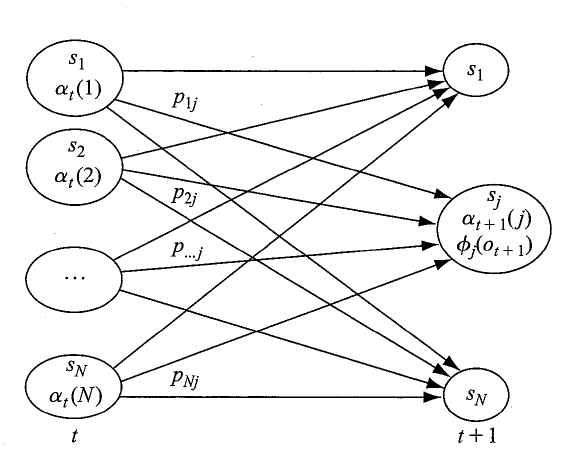
\includegraphics[width=3.5in]{f115}
\caption{前向算法的归纳}\label{fig:2}
\end{figure}

3.更新时间

令$t = t+1$,如果$t < T$,进入步骤2,否则进入步骤4。

4.算法终止

\begin{center}
$
P[O|\lambda]=\sum_{i=1}^N\alpha_T(i)=\sum_{i=1}^NP[O,q_T=s_i|\lambda]
$
\end{center}

前向算法需要$N(N+1)(T-1)+N$次乘法和$N(N-1)(T-1)$次加法,计算复杂度为$O(N^2T)$而不是$O(2TN^T)$。以前面的例子为例,$N=3,T=100$,前向算法需要900次计算,相比直接方法的$10^50$次计算要快得多。

后向算法是解决评价问题的一个双重问题。它需要定义一个后向概率变量$\beta_t(i)$:

\begin{center}
$
\beta_t(i)=P[o_{t+1},o_{t+2},...,o_T|q_t=s_i,\lambda]\quad t=1,...,T;s_i\in S
$
\end{center}

这就是说,$\beta_t(i)$是已知部分观测$o_{t+1},o_{t+2},...,o_T$,已知模型在时刻t时位于状态$s_i$。所以,$\beta_t(i)$可以如下表示:

\begin{center}
$
\begin{aligned}
\beta_t(i)=P[o_{t+1},o_{t+2},...,o_T|q_t=s_i,\lambda]\\
=\sum_{s_j\in S}P[o_{t+1},o_{t+2},...,o_T,q_{t+1}=s_j|q_t=s_i,\lambda]\\
=\sum_{s_j\in S}P[o_{t+1}|q_{t+1}=s_j]P[o_{t+2},...,o_T,q_{t+1}=s_j|q_t=s_i,\lambda]\\
=\sum_{s_j\in S}P[o_{t+1}|q_{t+1}=s_j]P[o_{t+2},...,o_T|q_{t+1}=s_j]P[q_{t+1}=s_j|q_t=s_i,\lambda]\\
=\sum_{j=1}^N\phi_j(o_{t+1})\beta_{t+1}(j)p_{ij}\quad t=1,...,T;i=1,...,N
\end{aligned}$
\end{center}

后向算法与前向算法的思想类似,但是是从右往左生成交织的。

1.初始化

$\beta_T(i)=1\quad 1\le i \le N$

2.归纳

\begin{center}
$
\beta_t(i)=\sum_{j=1}^N\phi_j(o_{t+1})\beta_{t+1}(j)p_{ij}\quad 1\le t\le T-1,1\le i \le N
$
\end{center}

3.更新时间

令$t=t-1$。如果$t>0$,转到步骤2,否则转到步骤4。

4.终止

\begin{center}
$
P[O|\lambda]=\sum_{i=1}^N\beta_1(i)\alpha_1(i)=\sum_{i=1}^N\beta_1(i)\pi_i\phi_i(o_1)
$
\end{center}

所谓的后向算法是从观测中来的,对于任意的t,$1\le t\le T$:

\begin{center}
$
P[O|\lambda]=\sum_{i=1}^N\beta_t(i)\alpha_t(i)
$
\end{center}


归纳的过程如图所示:

\begin{figure}[htbp]
\centering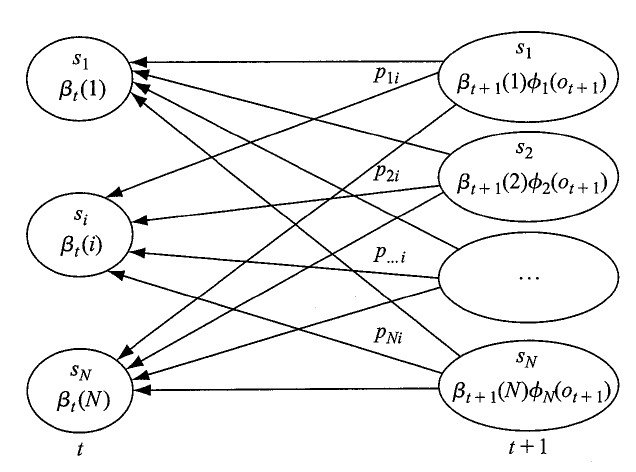
\includegraphics[width=3.5in]{f117}
\caption{后向算法的归纳}\label{fig:3}
\end{figure}


\subsection{解码问题与Viterbi算法}

第二个问题是解码问题,是已知观测序列O和已知模型$\lambda$,寻找最佳的状态序列。第一步是定义什么是最优的状态序列。一个可能的定义是最有可能产生观测序列的状态序列。因此,我们要找状态序列Q使得$P[Q|O,\lambda]$取得最大值。不幸的是,对于T种取值的挂车呢序列和N个状态的系统,一共有$N^T$中可能的序列Q。

考虑我们寻找单个的最可能的状态而不是作为一整个序列。对于每个时刻t,$1\le t\le T$,我们定义变量$\gamma_t(i)$:

\begin{center}
$
\begin{aligned}
\gamma_t(i)=P[q_t=s_i|O,\lambda]=\frac{P[q_t=s_i,O|\lambda]}{P[O|\lambda]}\\
=\frac{P[q_t=s_i,o_1,o_2,...,o_T|\lambda]}{P[O|\lambda]}\\
=\frac{P[q_t=s_i,o_1,o_2,...,o_t,o_{t+1},...,o_T|\lambda]}{P[O|\lambda]}\\
=\frac{P[q_t=s_i,o_1,o_2,...,o_t,o_{t+1},...,o_T|q_t=s_i,\lambda]P[q_t=s_i|\lambda]}{P[O|\lambda]}\\
=\frac{P[q_t=s_i,o_1,o_2,...,o_t|o_{t+1},...,o_T,q_t=s_i,\lambda]P[o_{t+1},...,o_T|q_t=s_i,\lambda]P[q_t=s_i|\lambda]}{P[O|\lambda]}\\
=\frac{P[q_t=s_i,o_1,o_2,...,o_t|q_t=s_i,\lambda]P[o_{t+1},...,o_T|q_t=s_i,\lambda]P[q_t=s_i|\lambda]}{P[O|\lambda]}\\
=\frac{P[q_t=s_i,o_1,o_2,...,o_t,q_t=s_i|\lambda]P[o_{t+1},...,o_T|q_t=s_i,\lambda]P[q_t=s_i|\lambda]}{P[O|\lambda]}\\
=\frac{\alpha_t(i)\beta_t(i)}{\sum_{i=1}^N\beta_t(i)\alpha_t(i)}
\end{aligned}$
\end{center}

其中最后一个等式由于之前我们得到的:

\begin{center}
$
P[O|\lambda]=\sum_{i=1}^N\beta_t(i)\alpha_t(i)
$
\end{center}

并且:

\begin{center}
$
\sum_{i=1}^N\gamma_t(i)=1
$
\end{center}

使得$\gamma_t(i)$是一个分布概率函数。因此个体在时刻t的最可能的状态为:

\begin{center}
$
q_t^*=arg \max_{1\le i \le N}\{\gamma_t(i)\}\quad 1 \le t\le T
$
\end{center}

因此这个方法对于给定的观察序列$O=\{o_1,o_2,...,o_T\}$会生成最优可能的状态序列$Q^*=\{q_1^*,q_2^*,...,q_T^*,\}$。然而,这种方案可能会生成一个不太可能的状态序列,因为它没有考虑状态转移概率。比如说,如果我们有一个劽包含两个相邻的状态$s_i$和$s_j$,转移概率$p_{ij}=0$,然后这个结果是一个无效的状态序列。一种有效的避免这种不可能序列的方法是Viterbi算法,是基于动态规划的。

\subsection{学习问题与Baum-Welch算法}

模型参数估计

\section{隐马尔科夫模型的类型}

介绍离散、连续HMM,和纯生隐马尔科夫过程

\section{有寂静状态的隐马尔科夫模型}

\section{隐马尔科夫过程延伸}

重点介绍HSMM隐半马尔科夫以及隐半马尔科夫的Viterbi算法

\end{document}